\subsection{Audio Engine des Samplers}\label{sec:audio-engine}

Die Hauptfunktionalität eines Audiosamplers ist das Aufnehmen und Abspielen von Audiosamples. 

Der gewählte PCM5102a Audio Codec verfügt lediglich über einen Ausgabestream, was eine Neubestellung eines Codecs mit In- und Output Stream erfordern würde.

Angesichts des ohnehin schon ambitionierten Featureumfangs und der damit verbundenen Zeitknappheit, wurde die Aufnahmefunktion \textbf{\hyperlink{lf-audiorecord}{LF04}} gestrichen, sodass der Prototyp zu einer reinen ``Sample-Playback`` Maschine wird. 

Das folgende Kapitel befasst sich mit der Implementierung und Ansteuerung der Audiowiedergabe über den Audio Codec und aller verbundenen DSP-Operationen.

Zunächst folgt eine Erläuterung des grundlegenden Signalfluss der Audioengine:

\subsubsection{Signalfluss der Audioengine}

Alle Audiosamples werden auf einer angeschlossen \textbf{SD Karte} persistent gespeichert. Diese werden dann immer stückweise mit dem \textbf{FATFS} Dateisystem, welches für eingebettete Systeme optimiert ist, in die Applikationslogik und somit den Audiopufferspeicher geladen. 

Von hier aus reicht die \textbf{DMA} den Buffer per \textbf{I2S} Protokoll an den \textbf{Audio Codec} weiter. 

Der Audio Codec wandelt die digitalen PCM Signale in eine analoges Signal mit Line-Level (\SI{\pm 1.7}{\volt_{rms}}).

\begin{figure}[h!]
	\centering
	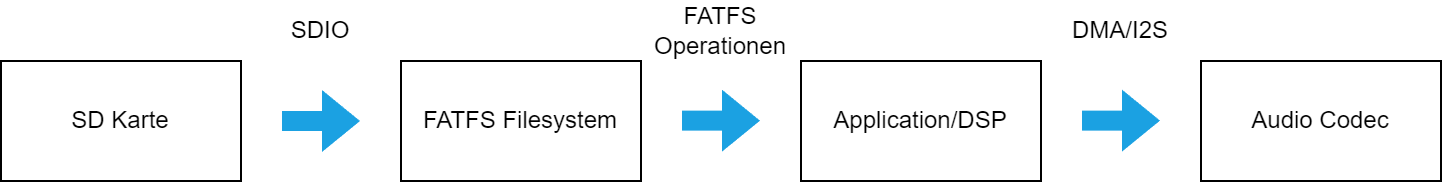
\includegraphics[width=0.9\textwidth]{images/08_durchfuehrung/audio/audio_signalflow.drawio.png}
	\caption{Digitaler Audio Signalfluss}
	\label{fig:audio_signalflow}
\end{figure}


\subsubsection{Latenzen}

Echtzeitfähigkeit ist ein kritischer Aspekt bei elektronischen Audioinstrumenten. 
Eine niedrige Latenz ist entscheidend, um rhythmisch präzise und ``tight`` zu spielen, besonders wenn mehrere Instrumente miteinander synchronisiert werden müssen.

Die maximale Latenz, die ein menschlicher Profimusiker noch akzeptieren kann, liegt bei etwa 20ms. Diese Richtwert basiert auf der Wahrnehmungsgrenze, bei der Musiker und Live-Performern keine signifikante zeitliche Verzögerung zwischen dem Triggern eines Samples und dessen tatsächlichem Output am Ausgang spüren. \cite{latency-experiment}

Um die Latenz auf ein Minimum zu reduzieren und sicherzustellen, dass elektronische Audioinstrumente reaktionsschnell und synchronisiert sind, können folgende Methoden angewendet werden:

\paragraph{Dimensionierung der Buffersize}\

Die erste Einstellungsmöglichkeit ist die \textit{Buffersize}.
Das ist die Größe (in Bytes) des Audiobuffers.
Je kleiner der Audiobuffer, desto öfter pro Sekunde gibt die DMA dessen Inhalt an den Audio Codec weiter.

Das bringt jedoch auch Performanceeinbußen mit sich: Bei kleinen Audiobuffern hat die CPU, je nach Komplexität der durchzuführenden DSP-Operationen, möglicherweise nicht genug Zeit, um den gesamten Buffer zu verarbeiten.
Ein nur teils verarbeiteter Buffer kann hörbare Knackser und Störgeräusche am Ausgangssignal verursachen.

Hier gilt es also, die kleinstmögliche Buffersize zu ermitteln, ohne dass Störgeräusche auftreten.
Nach Experimentieren hat sich ein Wert von \textbf{128 Bytes} als adäquat herausgestellt.

\paragraph{Verwendung von Double Buffering}\

Double Buffering ermöglicht es, Daten in einem Pufferspeicher zu verarbeiten, während gleichzeitig ein anderer Puffer für die Eingabe oder Ausgabe verwendet wird. Dies reduziert Verzögerungen und ermöglicht eine nahtlose Datenverarbeitung, da der Prozessor nicht auf das Ende einer Übertragung oder Berechnung warten muss, bevor er fortfahren kann. \cite{double-buffering}

\begin{figure}[H]
	\centering
	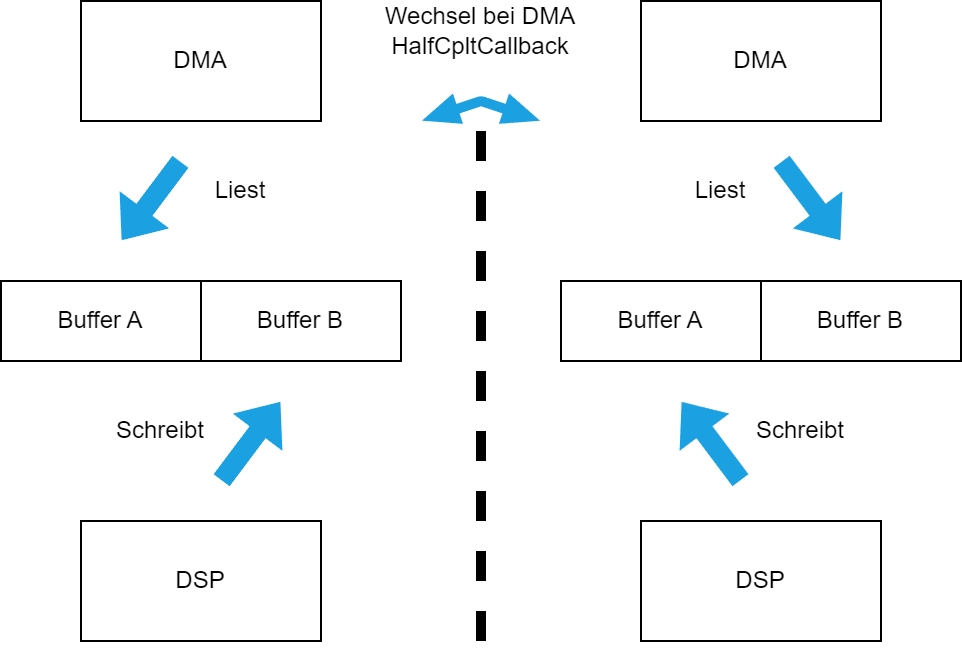
\includegraphics[width=0.6\textwidth]{images/08_durchfuehrung/audio/double_buffering.drawio.png}
	\caption{Double Buffering mit DMA und DSP}
	\label{fig:double_buffering}
\end{figure}


Bei I M A wird wird der Audiobuffer in zwei Hälften unterteilt.
Durch den Pointer \mintinline{c}|int16_t *outBufPtr|, welcher jeweils auf die erste oder zweiter Hälfte zeigt, wird mit der DSP die Hälfte bearbeitet, die gerade nicht von der DMA übertragen wird.

In den Callback-Funktionen \mintinline{c}|HAL_I2S_TxHalfCpltCallback()| und \mintinline{c}|HAL_I2S_TxCpltCallback()| wird der Pointer auf die jeweilige Hälfte des Buffers, also auf (wie in  \textbf{\autoref{fig:double_buffering}} beschrieben:
\textbf{Buffer~A} und \textbf{Buffer~B}) gesetzt.


\inputminted[firstline=28, lastline=31]{c}{../../f401_sd_card_audio_codec_test/Core/Src/audio.c}

\inputminted[firstline=40, lastline=43]{c}{../../f401_sd_card_audio_codec_test/Core/Src/audio.c}


Diese Callbacks, werden systembedingt aufgerufen, sobald die DMA die erste Hälfte oder den gesamten Buffer übertragen hat. Sie eignen sich daher sehr gut um den Pointer zu setzen.

Sobald das Flag \mintinline{c}|dma_dataReady == true| gesetzt ist, wird die nächste Bufferhälfte von der SD-Karte gelesen.

\paragraph{Latenzmessung}

Die Latenzmessung im Abschnitt \ref{test-latenzmessung} zeigt, dass die gemessene Latenz von Trigger Input bis Audioausgang mit \SI{6.7}{\milli\second} sehr zufriedenstellend ist, was ein erfolgreiches Zusammenspiel mit anderen elektronischen Instrumenten ermöglicht.


\subsubsection{PCM5102a und I2S}\label{sec:pcm5102a-und-i2s}

Ein sehr weit verbreitetes Protokoll zur digitalen Audioübertragung ist I2S. Viele Codecs, so auch der PCM5102a, unterstützen dieses Protokoll.

I2S (Inter-IC Sound) ist ein Standard für die digitale Übertragung von Audiodaten zwischen integrierten Schaltkreisen (ICs). Es wurde entwickelt, um die Kommunikation von digitalen Audiodaten zwischen verschiedenen Komponenten wie Mikrofonen, DACs (Digital-Analog-Wandler) und ADCs (Analog-Digital-Wandler) zu ermöglichen. \cite{i2s-reference}

Der PCM5102a erkennt komfortablerweise die eingehende Samplerate anhand der Bitclock.
Anders als bei vielen Audio Codecs ist keine zusätzliche Konfiguration des Chips über ein Kommunikationsprotokoll, wie I2C notwending.

Somit fallen auch keine Treiber für diesen Chip an, was die Einbindung sehr vereinfacht.

Die I2S Signale des PCM5102a sind:

\begin{itemize}
	\item \textbf{SCK (System Clock)}: Dieser Takt wird für den Betrieb des internen Digitalfilters und des DAC-Kerns verwendet. Er kann entweder extern bereitgestellt oder intern vom PCM5102a erzeugt werden.
	\item \textbf{BCK (Bit Clock)}: Dieser Takt signalisiert den Beginn jedes Bits im Datenwort. Der BCK wird verwendet, um die Daten auf der Datenleitung (DIN) zu takten.
	\item \textbf{LCK (Left/Right Clock)}: Auch als Word Select oder Frame Sync bekannt. Dieser Takt signalisiert den Beginn eines neuen Audioframes und zeigt an, ob die aktuellen Daten den linken oder rechten Kanal darstellen.
	\item \textbf{DIN (Digital Input)}: Dies ist die Datenleitung, über die die PCM-Audiodaten übertragen werden.
\end{itemize}

Der Einfachheit halber wird eine festgelegte Samplerate und nur Stereo-Samples verwendet.

\subsubsection{Audiostream von SD-Karte}
\label{sec:sd-card-audio}

Durch den sehr begrenzter RAM-Speicher des NUCLEO F401re Boards , ist es notwendig die Daten in Echtzeit von der SD-Karte zu streamen. Das setzt bei Stereo PCM Dateien, mit den gängigen Parametern, eine bestimmte Datenrate \( R \) voraus:

\begin{itemize}
	\item Abtastrate (Sampling Rate): 44.100 Hz (44,1 kHz)
	\item Bit-Tiefe: 16 Bit
	\item Kanäle: 2 (Stereo)
\end{itemize}

Die Datenrate \( R \) berechnet sich aus:

\[
R = \text{Sampling Rate} \times \text{Bit-Tiefe} \times \text{Anzahl der Kanäle}
\]



\[
R = 44{,}100 \, \text{Hz} \times 16 \, \text{bit} \times 2
\]

\[
R = 1{,}411{,}200 \, \text{bit/s} \approx 0.168 \, \text{MB/s}
\]


Theoretisch hätte eine Implementierung des FATFS-Dateisystems über SPI ausreichen müssen, um diese Datenraten zu bewältigen. 

Um die SDIO-Schnittstelle in das FATFS-Dateisystem zu integrieren, mussten zunächst Treiber entwickelt werden. Diese Treiber mappen die üblichen Dateioperationen wie \mintinline{c}|f_open()|, \mintinline{c}|f_read()| usw. über die SPI-Schnittstelle.

\begin{wrapfigure}{r}{0.3\textwidth} % Increase the width of the figure environment
	\fbox{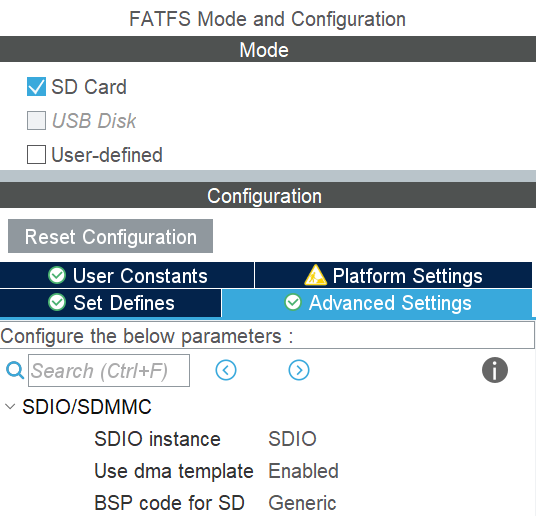
\includegraphics[width=0.3\textwidth]{images/08_durchfuehrung/audio/cubemx_sdio.png}}
	\caption{CubeMX FATFS SDIO Einbindung}
	\label{fig:cubemx_sdio}
\end{wrapfigure}

In der Praxis stellte sich jedoch heraus, dass der Audiobuffer nicht schnell genug gefüllt worden ist, was starke Knackser und Störgeräusche mit sich gebracht hat.

Dies erwies sich als äußerst vorteilhaft, da die SDIO-Implementierung zusammen mit FATFS direkt im Konfigurationstool von STM, \textbf{CubeMX}, ausgewählt werden kann. Die benötigten Treiber werden von CubeMX automatisch generiert und integrieren sich problemlos in das Dateisystem.

\subsubsection{Playback und Pitched Playback}

Der Audioplayer unterstützt das Abspielen von WAV-Dateien mit Tonhöhenanpassung. Dies wird durch die Verwendung von DMA zur Übertragung über I2S erreicht. Die Audiowiedergabe erfolgt mit dynamischer Anpassung der Abspielgeschwindigkeit, was eine Echtzeit-Tonhöhenänderung ermöglicht.

Die Funktion \mintinline{c}|wavPlayPitched(WavPlayer *player)| liest Audiodaten von der SD-Karte:

\mint{c}|bytesRead = fillHalfBufferFromSD(player, true);|

wobei die Funktion \mintinline{c}|fillHalfBufferFromSD()|, die Anzahl der benötigten Samples für den Buffer, dynamisch anhand der Abspielgeschwindigkeit errechnet.

\paragraph{Pitchfaktor}

Ein Pitchfaktor größer als 1.0 bedeutet, dass die Wiedergabegeschwindigkeit erhöht wird. Um diese höhere Geschwindigkeit zu kompensieren, müssen mehr Samples in den Puffer geladen werden. Das liegt daran, dass mehr Daten pro Zeiteinheit benötigt werden, um die schnellere Wiedergabe zu unterstützen.

Ein Pitchfaktor kleiner als 1.0 reduziert die Wiedergabegeschwindigkeit. In diesem Fall werden weniger Samples benötigt, weil sich die Daten im Puffer wiederholen. Das bedeutet, dass der Puffer nicht so schnell gefüllt werden muss, da die Audio-Daten langsamer abgespielt werden.

\paragraph{PCM-Stereocodierung}

Beim Füllen des Audiobuffers mit einem Pitchfaktor \( \neq 0 \) muss darauf geachtet werden, dass die PCM Stereo-Codierung korrekt beachtet wird. 
Im PCM Stereo-Format repräsentieren alle geraden Samples im Buffer den linken Kanal, während die ungeraden Samples den rechten Kanal darstellen.

Wenn der Pitchfaktor verändert wird, können Samples entweder übersprungen oder doppelt abgespielt werden. Dabei ist es entscheidend, dass die richtigen Samples für den linken und rechten Kanal ausgewählt werden. Der folgende Code sorgt dafür, dass diese Auswahl korrekt erfolgt:

\begin{minted}{c}
	leftReadIndex = (leftReadIndex + 1) & ~1;
	rightReadIndex = leftReadIndex + 1;
\end{minted}


\noindent
Hier ist eine detaillierte Erklärung dieser Operationen:

\begin{enumerate}
	\item \textbf{Sicherstellung eines geraden Indexes:} \\
	Der Code:
	\begin{quote}
		\mintinline{c}|leftReadIndex = (leftReadIndex + 1) & ~1;|
	\end{quote}
	sorgt dafür, dass \mintinline{c}|leftReadIndex| immer eine gerade Zahl ist. Zunächst wird \mintinline{c}|1| zu \mintinline{c}|leftReadIndex| addiert, um eine gerade Zahl zu erhalten. 
	
	Die bitweise UND-Operation mit \mintinline{c}|~1| (der negierten Zahl 1) entfernt das niedrigstwertige Bit von \mintinline{c}|leftReadIndex + 1|, wodurch der Wert zu einer geraden Zahl wird. 
	
	Zum Beispiel wird aus 5 (ungerade) 6 (gerade), und aus 7 (ungerade) wird ebenfalls 6 (gerade).
	
	\item \textbf{Berechnung des \mintinline{c}|rightReadIndex|:} \\
	Der Index für das rechte Sample wird durch die folgende Zeile berechnet:
	\begin{quote}
		\mintinline{c}|rightReadIndex = leftReadIndex + 1;|
	\end{quote}
	Nachdem \mintinline{c}|leftReadIndex| als gerade Zahl festgelegt wurde, ist \mintinline{c}|rightReadIndex| automatisch der nächste Index, der ungerade ist. Dies entspricht dem Format von PCM Stereo-Samples, bei dem gerade Indizes für den linken Kanal und ungerade Indizes für den rechten Kanal verwendet werden.
\end{enumerate}

Diese Schritte stellen sicher, dass die berechneten Indizes korrekt auf die im Stereo-PCM-Format erwarteten Positionen verweisen, indem sie sicherstellen, dass der Puffer die richtigen Daten für den linken und rechten Kanal enthält.


\subsubsection{Downsampling eines Audiochunks für die Verarbeitung von Audio durch das Neuronalen Netzes}
\label{sec:audio-downsampling}


Damit die proprietäre ``STM32\_AI\_AudioPreprocessing\_Library`` (Abschnitt \ref{sec:stm32-cube-ai}) die Audiodaten in Spektrogramme umwandeln kann, müssen die Daten zunächst ins korrekte Format gebracht werden. Für die Umwandlung erwartet die Library \SI{16}{\kilo\hertz} Samplerate, Mono Dateien.

In der Datei
\path{/f401_sd_card_audio_codec_test/Core/Src/audioPreprocessor.c}
finden sich alle Funktionen, die das Audiopreprocessing der Audiodatei für die Klassifizierung betreffen.

Die Funktion 
\mint{c}|uint32_t downsample_to_1024_samples(FIL *file, int16_t outChunk[NUM_SAMPLES_CHUNK_OUT])|
liest einen Audiochunk aus einer Datei von der SD Karte, konvertiert die Stereo-Samples in Mono und führt anschließend eine Abtastratenreduktion (Downsampling) durch. Die verarbeiteten Samples werden im \mintinline{c}|outChunk|-Buffer gespeichert. Die Funktion arbeitet blockweise und gibt die Anzahl der heruntergesampelten Samples zurück. 

Zunächst werden die Eingabedaten in den Puffer \mintinline{c}|inputChunk| eingelesen. Die Stereo-Samples werden durch Mittelung der linken und rechten Kanäle in Mono umgewandelt und in den Puffer \mintinline{c}|currentInBlockMono| geschrieben. Anschließend wird die Funktion \mintinline{c}|downsample_Block| aufgerufen, die die eigentliche Abtastratenreduktion und FIR-Filterung durchführt.

Die Funktion \mintinline{c}|downsample_Block| konvertiert die 16-Bit-Integer-Audiodaten in ein Fließkommaformat, führt FIR-Filterung und Dezimierung durch und konvertiert die gefilterten Samples zurück in das 16-Bit-Integer-Format. Die verarbeiteten Daten werden dann in den Zielpuffer geschrieben.

Um Aliasing beim heruntergesampleten Audiomaterial zu vermeiden, werden die benötigten Samples vor dem Downsampling mit einem FIR Highcut geglättet. 
Die Koeffizienten können mit Filterdesign-Softwares, wie \url{http://t-filter.engineerjs.com} generiert werden. Es wurde ein Filter mit 57 Koeffizienten gewählt, der eine gute Balance zwischen Performance und Ripple bietet. 
Wie in Abbildung \ref{fig:fir-filter} zu sehen, bietet der Filter ab \SI{16}{\kilo\hertz} eine recht steile Flanke bis \SI{-45}{\deci\bel} Abschwächung.

\begin{figure}[h!]
	\centering
	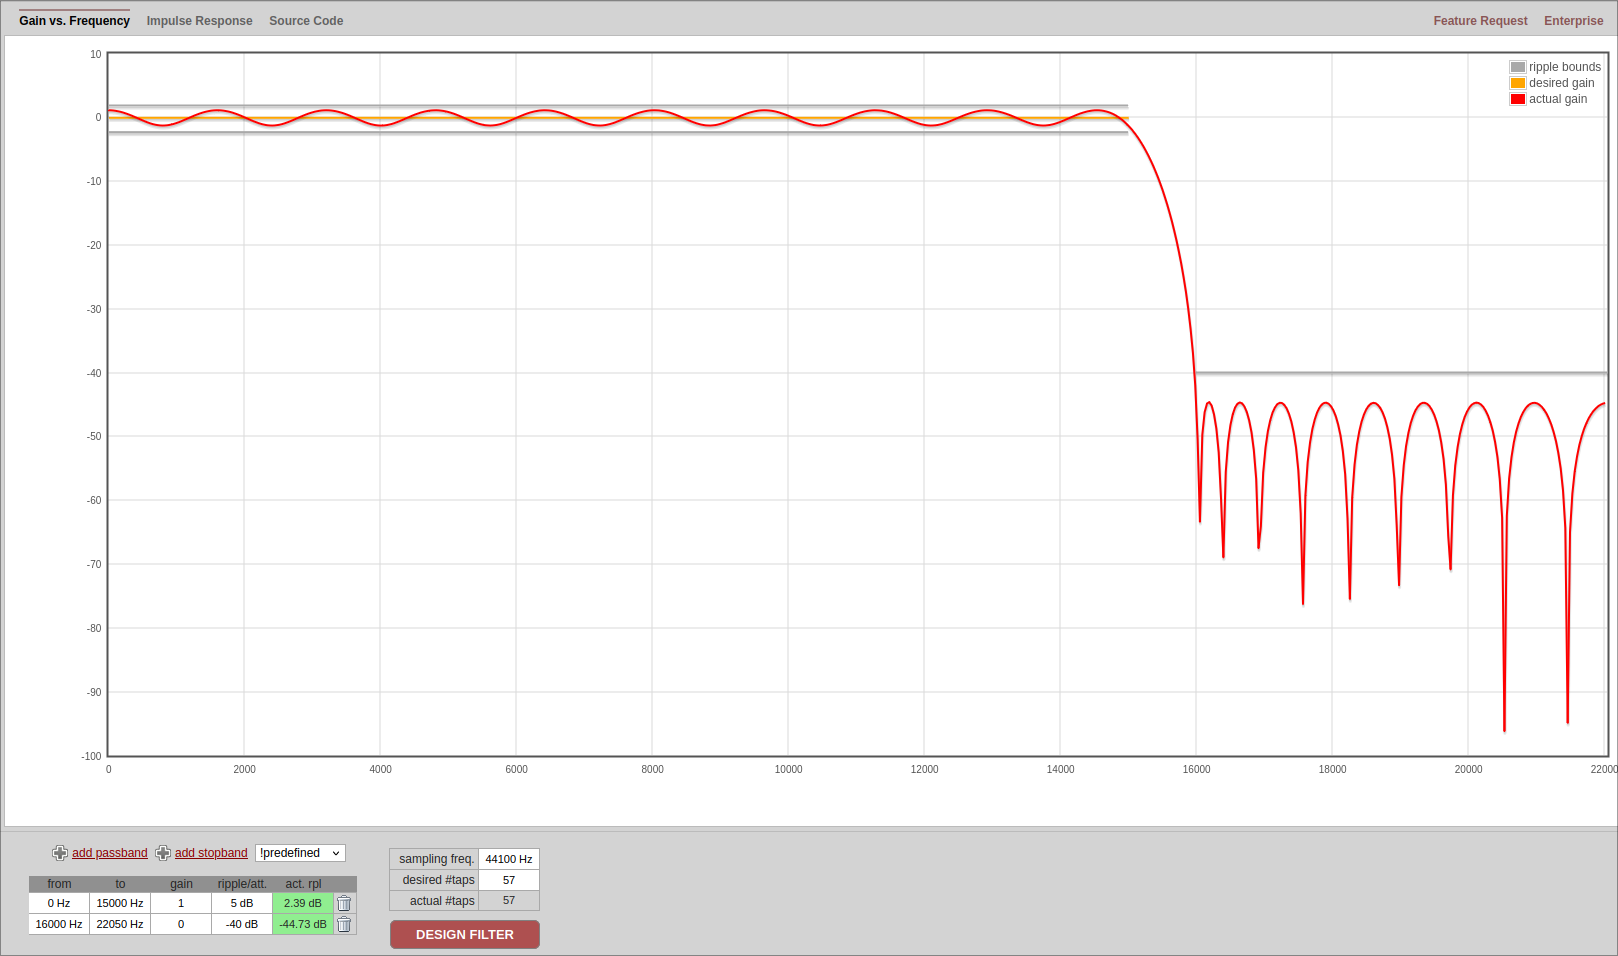
\includegraphics[width=0.6\textwidth]{images/08_durchfuehrung/audio/fir_lowpass.png}
	\caption{Anti-Aliasing FIR Lowpass Filter}
	\label{fig:fir-filter}
\end{figure}

Die Open Source CMSIS DSP Library \cite{cmsis-dsp}, für ARM Architekturen, bietet direkt eine optimierte Funktion, welche die FIR-Filterung, sowie das eigentliche Downsampling kombiniert: \mintinline{c}|arm_fir_decimate_f32|.
Diese Funktion akzeptiert jedoch nur ganze Downsampling-Faktoren.

Der benötigte Downsampling-Faktor ist:

\[
\frac{44{,}100 \text{ Hz}}{16{,}000 \text{ Hz}} = 2{,}75625
\]

Daher wird auf \(3.0\) aufgerundet, um einen ganzzahligen Faktor zu erreichen. 
Die resultierende neue Samplerate des heruntergesampleten Samples beträgt:

\[
\frac{44{,}100 \text{ Hz}}{3.0} = 14{,}700 \text{ Hz}
\]


